\normaltrue
\correctionfalse

%\UPSTIidClasse{11} % 11 sup, 12 spé
%\newcommand{\UPSTIidClasse}{11}

\exer{Mouvement R  $\star$ \label{C2:07:02} }
\setcounter{numques}{0}
\UPSTIcompetence[2]{C2-07}

\index{Compétence C2-07}
\index{Principe fondamental de la statique}
\index{PFS}
\index{Mécanisme à 1 rotation}
\ifcorrection
\else
\textbf{Pas de corrigé pour cet exercice.}
\fi

\ifprof
\else
Soit le mécanisme suivant. On a $\vect{AB}=R\vect{i_1}$ avec $R=\SI{20}{mm}$. La liaison pivot est motorisée par un moteur dont l'action mécanique sur \textbf{1} est donnée par $\vect{C_m}=C_m \vect{k_0}$.
On note $m_1$ la masse du solide 1 et $B$ son centre d'inertie. 
 La pesanteur est telle que $\vect{g}=-g\vect{j_0}$.
%On note $m_1$ la masse du solide 1, $B$ son centre d'inertie et $\inertie{G}{1}=\matinertie{A_1}{A_1}{A_1}{0}{0}{0}{\bas{1}}$.

\begin{center}
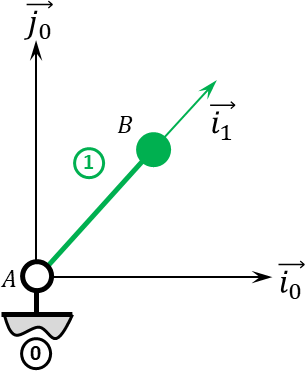
\includegraphics[width=\linewidth]{02_R_01}
\end{center}
\fi

\question{Réaliser le graphe d'analyse en faisant apparaître l'ensemble des actions mécaniques.}
\ifprof

\begin{center}
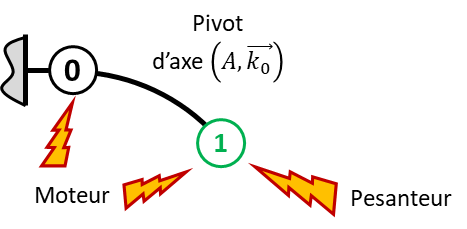
\includegraphics[width=.4\linewidth]{02_R_01_c}
\end{center}
\else
\fi

On donne 
%$\torseurstat{F}{0}{1}=\torseurl{X_{01}\vi{1}+Y_{01}\vj{1}+Z_{01}\vk{1}}{L_{01}\vi{1}+M_{01}\vj{1}}{A}$,
$\torseurstat{F}{\text{pes}}{1}=\torseurl{-m_1g\vj{0}}{\vect{0}}{B}$ et
$\torseurstat{F}{\text{Mot}}{1}=\torseurl{\vect{0}}{C_m\vk{0}}{A}$.

On isole \textbf{1} et on réalise un théorème du moment statique en $A$ en projection sur $\vk{0}$.

\question{Donner l'équation d'équilibre de la pièce \textbf{1}.}
\ifprof

\begin{itemize}
\item On isole \textbf{1}.
\item Bilan des actions mécaniques : 
\begin{itemize}
\item $\torseurstat{F}{0}{1}=\torseurl{X_{01}\vi{0}+Y_{01}\vj{0}}{\vect{0}}{A}$;
\item $\torseurstat{F}{\text{Mot}}{1}=\torseurl{\vect{0}}{C_m\vk{0}}{A}$;
\item $\torseurstat{F}{\text{pes}}{1}=\torseurl{-m_1g\vj{0}}{\vect{0}}{B}$ et 
$\vectm{A}{\text{pes}}{1} = \vectm{B}{\text{pes}}{1} + \vect{AB}\wedge -m_1g\vj{0}$.
\end{itemize}
\item 
\end{itemize}
\else
\fi


\question{Déterminer l'ensemble des inconnues de liaisons.}
\ifprof
\else
\fi

\ifprof
\else
%\footnotesize
%\begin{center}
%\begin{tabular}{|p{.9\linewidth}|}
%\hline
%Indications :
%\begin{enumerate}
%\item .
%\item $\torseurstat{F}{0}{1}=\torseurl{X_{01}\vi{1}+Y_{01}\vj{1}+Z_{01}\vk{1}}{L_{01}\vi{1}+M_{01}\vj{1}}{A}$,
%$\torseurstat{F}{\text{pes}}{1}=\torseurl{-m_1g\vj{0}}{\vect{0}}{B}$,
%$\torseurstat{F}{\text{Mot}}{1}=\torseurl{\vect{0}}{C_m\vk{0}}{A}$.
%\item $\torseurstat{F}{0}{1}=\torseurl{X_{01}\vi{1}+Y_{01}\vj{1}}{M_{01}\vj{1}}{A}$,
%$\torseurstat{F}{\text{pes}}{1}=\torseurl{-m_1g\vj{0}}{\vect{0}}{B}$,
%$\torseurstat{F}{\text{Mot}}{1}=\torseurl{\vect{0}}{C_m\vk{0}}{A}$.
%\item TMS en $A$ en projection sur $\vk{0}$.
%\end{enumerate} \\ \hline
%\end{tabular}
%\end{center}
%\normalsize
\begin{flushright}
\footnotesize{Corrigé  voir \ref{C2:07:02}.}
\end{flushright}%
\fi